A \textbf{genetic algorithm} is a search algorithm in which successor states are generated by picking two parent states, instead of choosing one state from the neighborhood of
the current solution. Before moving on, we define some common terms about genetic algorithms. \vspace{3.5pt}

Genetic algorithms are inspired by the process of \textbf{evolution}, composed as follows:
\begin{itemize}
    \renewcommand{\labelitemi}{-}
    \item \textbf{Inheritance}: offspring resemble their parents.
    \item \textbf{Adaptation}: organisms are suited to their habitats.
    \item \textbf{Natural selection}: new types of organisms emerge and those that fail to change are subject to extinction.
\end{itemize}

It's important to note that the specific terminology for genetic algorithms differs from that used for local search algorithms, it becomes:
\begin{itemize}
    \renewcommand{\labelitemi}{-}
    \item Each single solution defines a \textbf{genotype}.
    \item The set of solutions is called \textbf{population}.
    \item Chromosomes are made of units called \textbf{genes}.
    \item The domain of values of a gene is composed of \textbf{alleles}.
\end{itemize} \vspace{3.5pt}

Having described the terminology of genetic algorithms, let's examine how they work. Genetic algorithms begin with a set of $k$ randomly generated states, representing the
\textbf{population}. Each state, or \textbf{genotype}, is represented as a string over a finite alphabet, most commonly, a string of 0s and 1s. For example, in the image
below, which shows the 8-queens problem, each state can be specified as the positions of the 8 queens. Therefore, each genotype is an array of eight elements and the current 
position assumed by the queen will be inserted within each cell. \vspace{3.5pt}
\begin{center}
    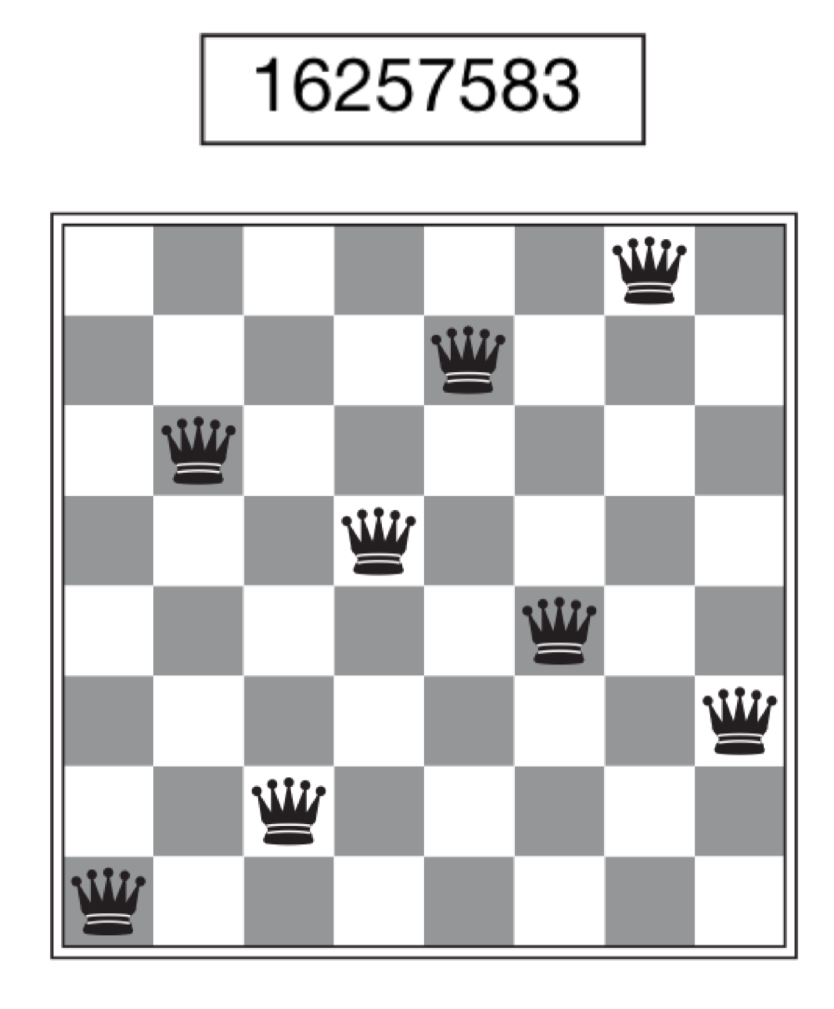
\includegraphics[width=0.3\textwidth]{img/img6.png} \\
    \scriptsize Here we are ordering the genotype by columns. It can also be expressed via rows.
\end{center} \vspace{3.5pt}
Defined the representation of states, each of them is rated by a \textbf{fitness function}, such that the algorithm will take some genotypes for the production of the next 
generation of states. A fitness function should return higher values for better states, so, for the 8-queens problem we use the number of non-attacking pairs of queens. In 
this case, the probability of being choosen for reproducing is directly proportional to the \textbf{fitness score}. \vspace{3.5pt}

According to the fitness probabilities, pairs of genotypes are taken from the population and then combined for the reproduction. Hopefully, if the parent genotypes are great 
solutions, then the offspring generated might be a better solution than before, but it's not guaranteed. For each pair, a \textbf{crossover point} is chosen randomly 
from the position in the string. As in the example introduced, portions of the array representation are swapped. \vspace{3.5pt}

Finally, the offspring generated is subject to a random \textbf{mutation}, one of the digit that composed the array representation is changed; this corresponds to choosing a 
queen randomly and moving it to a random cell. A visual summary on the main steps of genetic algorithms is shown below. \vspace{3.5pt}
\begin{center}
    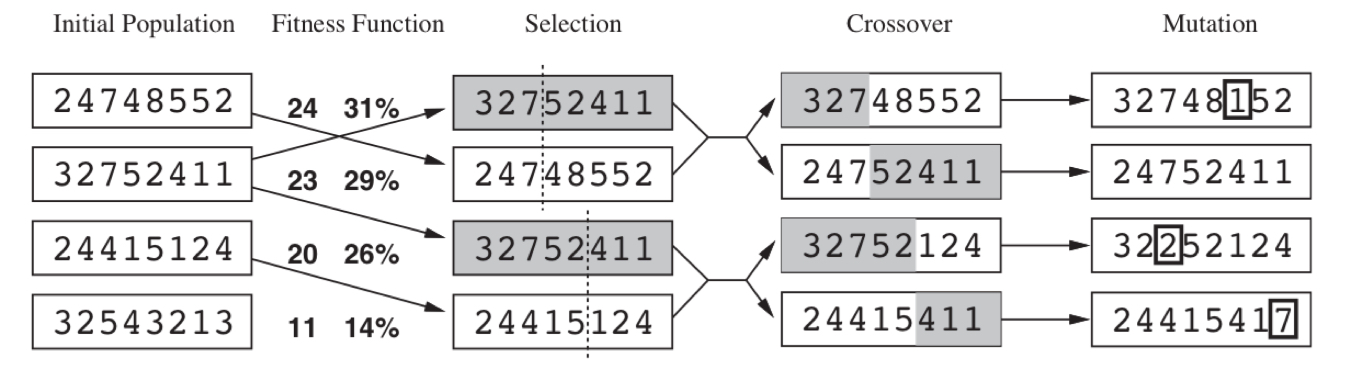
\includegraphics[width=0.9\textwidth]{img/img7.png}
\end{center} \vspace{3.5pt}

Replacing all the population each time a new generation is created, it determines a method that is computationally easier than any other algorithm seen so far; we substitute 
the old population with a new one, and that's it. However, this behavior can cause a major disadvantage: good solutions are not maintained in the new population. Generally, 
to avoid this, the best $n$ individuals from the new and old population are kept, hoping that the next generation can achieve a greater result. \vspace{3.5pt}

Despite genetic algorithms being extremely simple and easy to associate with different types of purposes, they are influenced by two main constraints:
\begin{itemize}
    \renewcommand{\labelitemi}{-}
    \item It can be a little too simple according to the operations performed.
    \item We have to tune a lot of parameters; remember the representation of genotypes, results coming from mutation, permutation and selection or the crossover point.
\end{itemize}